\chapter{Methodology} 
\label{chap:methodology}
This chapter describes the experimental setup used to evaluate the \acrfull{s6} model for temporal event spotting in football video. The section details the computing infrastructure, data preprocessing, and feature extraction pipeline, as well as model architectures, training protocols, and evaluation metrics. All aligned with the research questions (\autoref{sec:research_questions}).



\section{Notation}
\label{sec:notation}
Let
\begin{itemize}
  \item $V=\{x_t\}_{t=1}^T$ be an input video of $T$ frames,
  \item $\mathcal{C}=\{1,\dots,12\}$ the set of action classes,
  \item $\mathcal{Y}=\{(t_i,c_i)\}_{i=1}^N$ the ground-truth annotations (timestamp $t_i$, class $c_i$),
  \item $\hat{\mathcal{Y}}=\{(\hat t_j,\hat c_j,\hat s_j)\}_{j=1}^M$ the model's predicted timestamps, classes, and confidence scores.
\end{itemize}
We consider a prediction $(\hat t_j,\hat c_j)$ correct if $\hat c_j=c_i$ and $|\hat t_j - t_i|\le\Delta$, where $\Delta$ is a fixed tolerance window (e.g.\ 1 s). Performance is measured by \acrfull{map} over all classes under the chosen $\Delta$.


\section{Datasets}
\label{sec:method_datasets}

\subsection{THUMOS-14}
\label{ssec:method_thumos14}
The THUMOS-14 dataset \cite{dataset:thumos} is a widely used benchmark for temporal action localization. According to \hyperlink{https://paperswithcode.com/dataset/thumos14-1}{Papers With Code}, it is the most popular in the temporal action localization category as of the 29th of May 2025. It consists of over 13,000 temporally annotated action instances distributed across 20 distinct action classes. Its primary focus is on sports activities. The dataset provides untrimmed videos. It is suitable for evaluating models on their ability to detect and localize actions within more extended video sequences. 

Key characteristics of THUMOS-14 include:
\begin{itemize}
    \item \textbf{Action Classes}: 20 diverse action categories.
    \item \textbf{Video Content}: Primarily sports-related, sourced from YouTube.
    \item \textbf{Annotations}: Provides temporal annotations (start and end times) for action instances in the validation and test sets.
    \item \textbf{Dataset Split}: Includes training, validation, and testing sets. The validation set contains 1010 videos, and the test set contains 1574 videos. Among these, there are 432 videos with temporal annotations, comprising 220 validation videos and 212 labeled test videos. 
    \item \textbf{Evaluation}: Performance is typically measured using \acrfull{map} at various \acrfull{iou} thresholds.
\end{itemize}

In this work, THUMOS-14 is relevant as it serves as a benchmark for many temporal action localization models, including \acrshort{vms} and RDFA-S6. The \acrshort{vms} implementation used in this study provides preprocessing scripts and configurations tailored for THUMOS-14.

\subsection{SoccerNet-V2}
\label{ssec:dataset_soccernet}

The SoccerNet-V2 dataset \cite{deliege_soccernet-v2_dataset_2021} comprises video recordings of 7 professional football matches, along with fine-grained annotations for 12 action classes. It provides:
\begin{itemize}
    \item 7 full matches (90 min each) at 25 fps.
    \item Timestamped action labels for spotting tasks.
    \item Team annotations for each event.
    \item Publicly accessible annotations via HuggingFace\footnote{\url{https://huggingface.co/datasets/SoccerNet/SN-BAS-2025}}.
    \item An action approximately every 3 seconds. 
    \item Twelve football event classes:
        \begin{center}
            \begin{tabular}{llll}
                Pass & Drive & Header & High Pass \\
                Out & Cross & Throw In & Shot \\
                Ball Player Block & Player Successful Tackle & Free Kick & Goal
            \end{tabular}
        \end{center}
\end{itemize}

A non-disclosure agreement locks the video data. One can access annotations to seven out of nine annotated games, while the last two pertain to the challenge. These nine games come from the second tier of English football, the Championship. The games were played in October 2019. The specific games are:

\begin{itemize}
    \item 2019-10-01 - Leeds United - West Bromwich
    \item 2019-10-01 - Hull City - Sheffield Wednesday
    \item 2019-10-01 - Brentford - Bristol City
    \item 2019-10-01 - Blackburn Rovers - Nottingham Forest
    \item 2019-10-01 - Middlesbrough - Preston North End
    \item 2019-10-01 - Stoke City - Huddersfield Town
    \item 2019-10-01 - Reading - Fulham
    \item 2019-10-02 - Cardiff City - Queens Park Rangers
    \item 2019-10-01 - Wigan Athletic - Birmingham City
\end{itemize}

The authors claim that the first four games serve as training games, while the fifth is a validation game. The sixth and seventh games are test games used for testing purposes, while the last two games do not have public annotations. They are the challenge games, as mentioned above. All videos are in the *.mkv file format. 

\begin{figure}
    \centering
    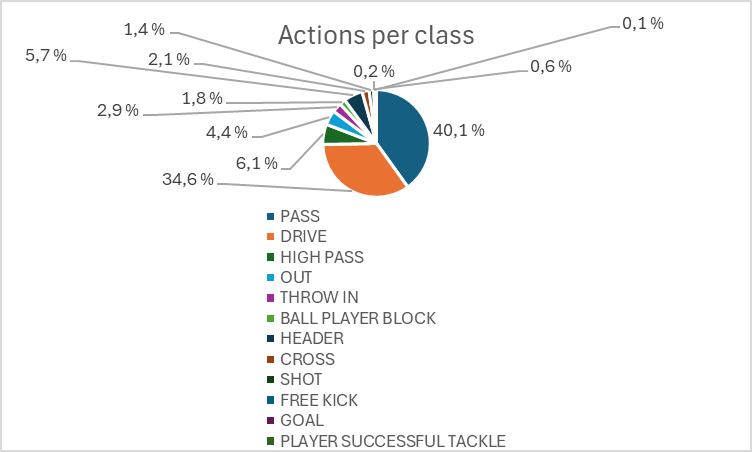
\includegraphics[width=1\linewidth]{figures/actions_per_class_2.png}
    \caption{Action distribution for different classes in the SoccerNet dataset for action ball spotting. }
    \label{fig:soccernet_dist}
\end{figure}

\begin{table}
    \centering
    \begin{tabular}{lr}
        \toprule
        Action                    & Count \\
        \midrule
        PASS                      & 4985  \\
        DRIVE                     & 4300  \\
        HIGH PASS                 & 761   \\
        HEADER                    & 713   \\
        OUT                       & 551   \\
        THROW IN                  & 362   \\
        CROSS                     & 261   \\
        BALL PLAYER BLOCK         & 223   \\
        SHOT                      & 169   \\
        PLAYER SUCCESSFUL TACKLE  & 74    \\
        FREE KICK                 & 21    \\
        GOAL                      & 13    \\
        \bottomrule
    \end{tabular}
    \caption{Soccer actions and their counts}
    \label{tab:soccer_actions}
\end{table}


\cref{sec:preprocessing} provides a more in-depth explanation of SoccerNet-label creation. The data is similar to THUMOS labels, aligning with the expected input of the \acrshort{vms} model.

\cref{tab:soccer_actions} and \cref{fig:soccernet_dist} show the distribution of 12,433 labels among the actions. There is an uneven distribution of actions. The evaluation does not consider the lopsided distribution when evaluating the \acrshort{map}.

The SoccerNet dataset contains 500 videos with temporal annotations related to an earlier challenge. There are 17 action classes.
\begin{itemize}
    \item Penalty
    \item Kick-off
    \item Goal
    \item Substitution
    \item Offside
    \item Shots on target
    \item Shots off target
    \item Clearance
    \item Ball out of play
    \item Throw-in
    \item Foul
    \item Indirect free-kick
    \item Direct free-kick
    \item Corner
    \item Yellow card
    \item Red card
    \item Yellow->red card
\end{itemize}

The actions are associated with a single timestamp, and their action density is lower compared to the new dataset. The videos are available behind the NDA, and they also provide extracted features for these. 

\section{Data Preprocessing \& Feature Extraction}
\label{sec:preprocessing}

The SoccerNet-V2 dataset \cite{deliege_soccernet-v2_dataset_2021} serves as the base for the experiments. Videos are split into non-overlapping clips $V_k=\{x_t\}_{t=1}^{T_c}$ of fixed duration $T_c=60\!\times\!25$ frames (60\,s at 25\,fps). The hyperparameter search used a 70-30 split. Training and validation used an 80-20 split. The 80-20 split matches the official publication. 70-30 matches a PyTorch recommendation in the docs \footnote{\url{https://docs.pytorch.org/docs/stable/data.html}. Retrieved the 13th of May}.

\lstinputlisting[
    caption={Script to change the label-file to the THUMOS-14 format.},
    label=lst:jsonfile,
    language=Python
]{listings/sn_to_json.py}

The duration key is unnecessary in the case of temporal action localization, as shown in the \autoref{lst:uselessduration}, which sets a default value if the duration is undefined. The video clip at the end of each half, $V_{N}$, has a $T_c$ that refers to the length of the clip. \acrfull{vms} handles different-length inputs. 

\lstinputlisting[
    caption={Part of \acrshort{vms} code used to determine the duration to be pointless. },
    label=lst:uselessduration,
    language=Python
]{listings/useless_duration.py}

Each clip $V_k$ is fed through the pre‐trained \acrshort{vmae} encoder (\cref{ssec:videomae_v2}) to extract a feature embedding
\[
z_k = \mathrm{VideoMAE\text{-}V2}(V_k)\;\in\;\mathbb{R}^D.
\]
These $D$‐dimensional vectors serve as inputs to the downstream temporal MAMBA model. \acrshort{idun} stores vectors as \textit{*.pt} files. Storing the vectors offline eliminates redundant computations, reduces storage requirements, and significantly lowers training times. 

When splitting the football videos into clips, we adopted a simplified protocol rather than seeking an optimal one. Future research could explore overlapping windows, adaptive clip boundaries, or dynamic segmentation schemes to mitigate boundary artifacts and improve temporal event localization. The scope of the literature study did not cover these topics.

Despite its effectiveness in learning meaningful spatiotemporal representations, \acrfull{vmae} incurs substantial computational overhead and is not managed. The dual-stage masking strategy yields robust feature embeddings in which up to 90 \% of video tokens are masked. However, it also increases the number of model parameters and the complexity of each forward pass. In practice, processing a single 60s clip at 25 fps requires on the order of tens of gigaflops \cite{wang_videomae_2023}. \acrshort{vmae} extracts and stores embeddings offline to mitigate these resource requirements. The heavy compute footprint of \acrshort{vmae} motivates the exploration of more lightweight architectures or more aggressive token reduction techniques in future work.

\acrshort{vmae} has been pre-trained on the large-scale Kinetics dataset. Consequently, its learned representations capture broad spatiotemporal patterns common to various athletic activities not explicitly tailored to football. While this generic pretraining supports robust feature extraction across multiple sports domains, specialized fine-tuning on football video may improve temporal event localization performance. Future work should explore domain-specific adaptation using dedicated football datasets to bridge the gap between Kinetics footage and match-level footage. 

InternVideo is the foundation for the comparative experiment, which evaluates 1,408-dimensional feature vectors extracted by a Kinetics-pretrained model against 3,302-dimensional embeddings generated. Both architectures originate from the same research group that developed \acrshort{vmae}. InternVideo is a bigger, still open-source framework.



\section{Model Architectures}
\label{sec:model_architectures}

\subsection{VideoMAE-V2}
\label{ssec:videomae_v2}

\subsubsection{Masking}

An encoder-decoder masking setup tokenizes input video frames into spatio-temporal patches. A binary mask tensor \(M\in\{0,1\}^{T\times H\times W}\) with masking ratio \(r\) is generated, where
\[
\sum_{t,h,w} M_{t,h,w} = r\,T\,H\,W.
\]
The visible patches \(x_\text{vis}\) are obtained by
\[
x_\text{vis} = x \,\odot\,(1 - M)\,,
\]
and fed into a lightweight transformer encoder \(E\). The decoder \(D\) takes the encoder output, plus positional embeddings and mask tokens, and attempts to reconstruct the original video:
\[
\hat{x} = D\bigl(E(x_\text{vis}),\,\text{mask\_tokens}\bigr).
\]
The training process minimizes the reconstruction loss only over masked positions:
\[
\mathcal{L} \;=\; \bigl\lVert\,M \,\odot\,(x - \hat{x})\bigr\rVert_2^2.
\]


\acrfull{vmae} by \textcite{wang_videomae_2023} is a self‑supervised masked autoencoder designed to preprocess and compress large‑scale video data before downstream experiments. Building on the original VideoMAE\cite{tong_videomae_2022}, it introduces a dual‑stage masking schedule: 

\begin{itemize}
    \item \emph{Sparse spatiotemporal masking} in early epochs to encourage global context learning over long clips,
    \item \emph{Dense tube masking} in later epochs to refine local motion representations.
\end{itemize}

VideoMAE has three components: embedder, encoder, and decoder. VideoMAE uses cube embedding \(\Phi_{emb}\) to transform frames into sequences of tokens. It designs a tube masking strategy with a ratio of \(\rho \simeq 90\%\). A vanilla \acrshort{vit} backbone encodes the visible tokens. A decoder reconstructs the masked patches using another \acrshort{vit}\cite{wang_videomae_2023}. 

By dynamically varying the masking granularity, VideoMAE‑V2 achieves:
\begin{itemize}
    \item 2× faster convergence compared to VideoMAE,
    \item linear scaling to billion‑parameter models,
    \item robust transferability across action recognition, temporal localization, and segmentation tasks\cite{wang_videomae_2023}.
\end{itemize}

Pre-extraction of \acrshort{vmae} embeddings significantly reduces storage and computational demands. Saving compact feature vectors instead of raw video sequences lowers I/O overhead and accelerates data loading. This approach decouples frame encoding from model training, enabling more rapid and iterative experimentation. As a result, overall training time decreases, and resource utilization improves.

\subsection{\acrfull{s6}}
\label{ssec:s6}

\acrfull{ssm} offers a continuous-time representation of sequential data via a latent state \(h(t)\in\mathbb{R}^N\):
\begin{align}
    \frac{\mathrm{d}h(t)}{\mathrm{d}t} &= A\,h(t) + B\,x(t),  \label{eq:ssm_continuous1}\\
    y(t) &= C\,h(t),                                    \label{eq:ssm_continuous2}
\end{align}
where \(x(t)\in\mathbb{R}^d\) is the input, \(y(t)\in\mathbb{R}^m\) the output, and \(A\in\mathbb{R}^{N\times N}, B\in\mathbb{R}^{N\times d}, C\in\mathbb{R}^{m\times N}\) are learned parameters.  Discretizing these equations with step size \(\Delta\) yields
\begin{align}
    \bar A &= \exp(\Delta\,A), 
    & 
    \bar B &= \bigl(\exp(\Delta\,A)-I\bigr)A^{-1}B,\\
    h_k &= \bar A\,h_{k-1} + \bar B\,x_k, 
    &
    y_k &= C\,h_k,
    \quad k=1,2,\dots
\end{align}

VideoMamba \cite{li_videomamba_2024} builds on this framework with a \emph{Selective Scan} (\acrshort{s6}) core. Its parameters \((\Delta, A,B,C)\) control:
\begin{itemize}
    \item \(\Delta\): temporal resolution of the recurrence,
    \item \(A\): continuous dynamics matrix,
    \item \(B,C\): input and output mappings.
\end{itemize}

By preserving a compact hidden state, Mamba approximates long-range dependencies akin to self-attention but with only \(\mathcal{O}(L)\) time/memory cost rather than \(\mathcal{O}(L^2)\) of the \acrfull{vit}.  


\subsubsection{Mamba Block}

\begin{figure}[h]
    \centering
    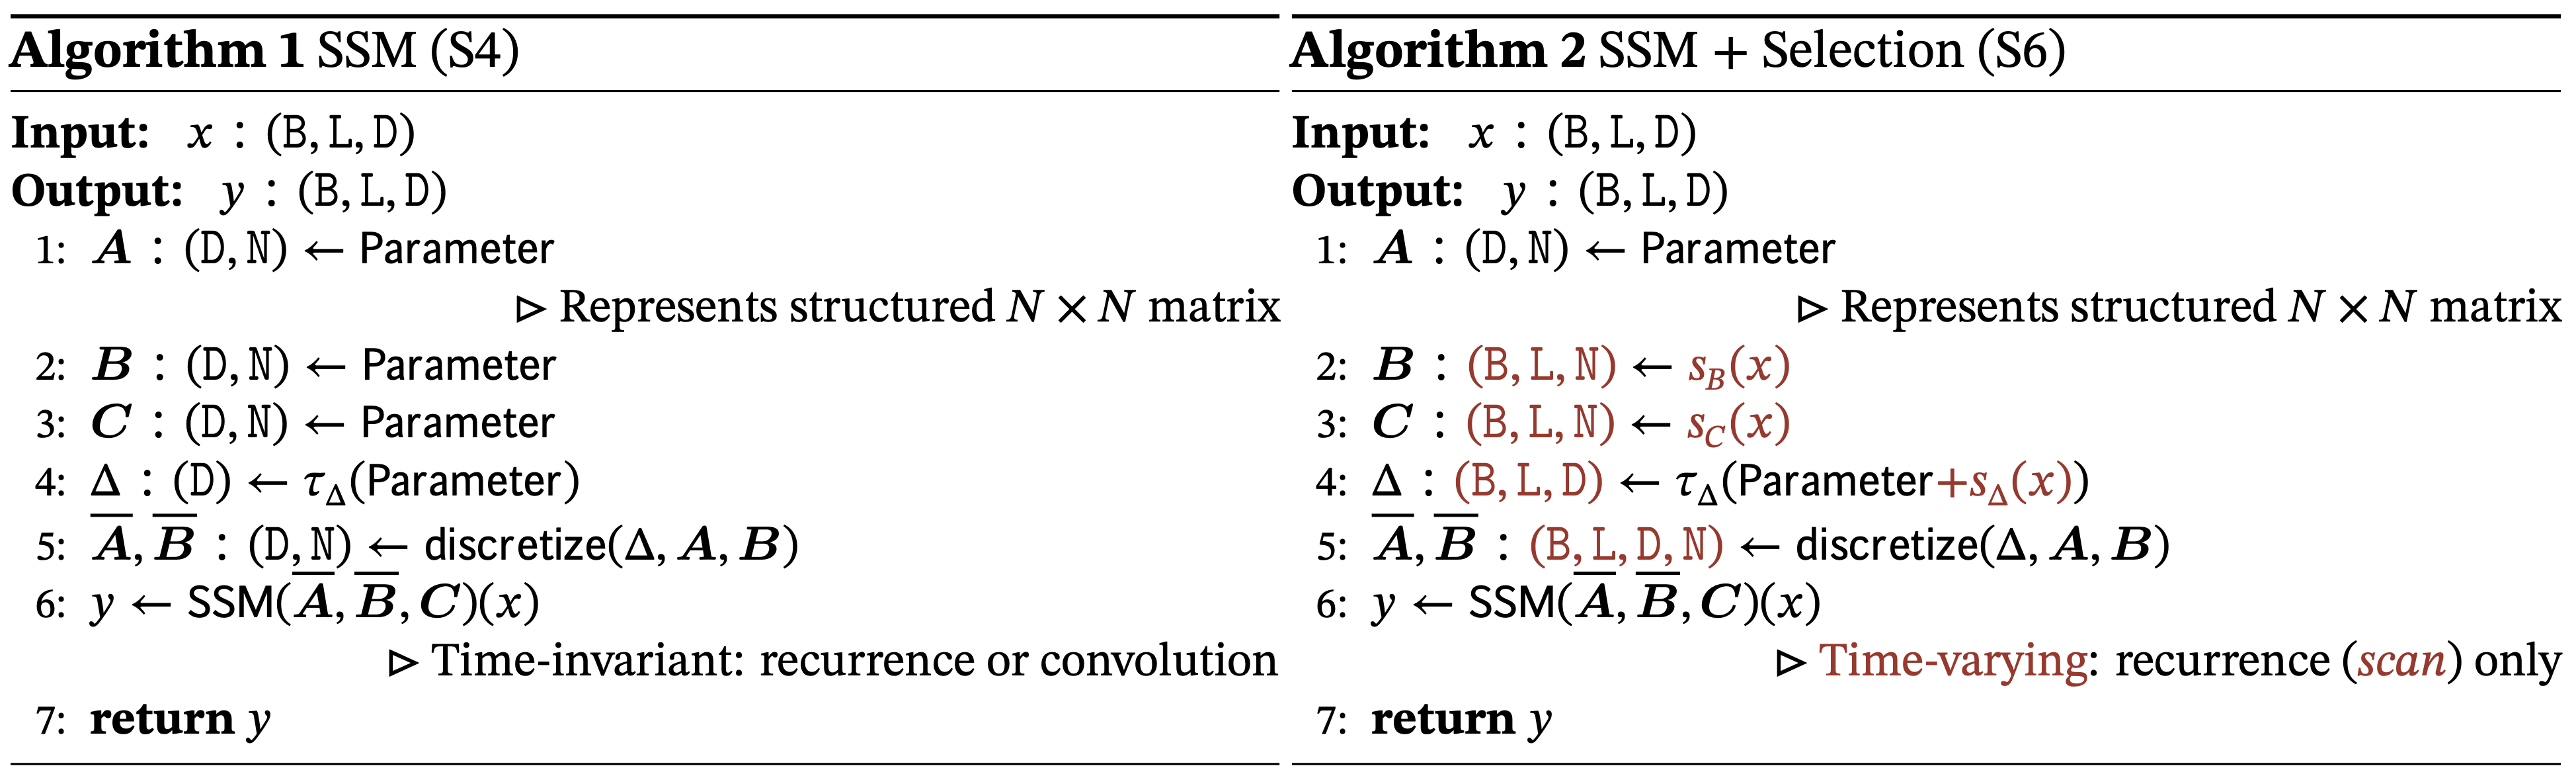
\includegraphics[width=1\linewidth]{figures/mamba_algorithm.png}
\end{figure}

Mamba\cite{gu_mamba_2024} creates a selection mechanism for compressing context into a smaller state. It introduces input-dependent parameters to allow the model to either keep or discard information. The approach enables linear scaling with respect to sequence length. The algorithm utilizes functions to update the \(B\) and \(C\) matrices, as described in the algorithm design by \textcite{gu_mamba_2024}. The Mamba blocks are hardware-aware; they use kernel fusion, parallel scan, and recomputation to address the limitations of Limited Time Invariance. Fast SRAM directly loads SSM into memory on \acrshort{gpu}s. 

\begin{figure}
    \centering
    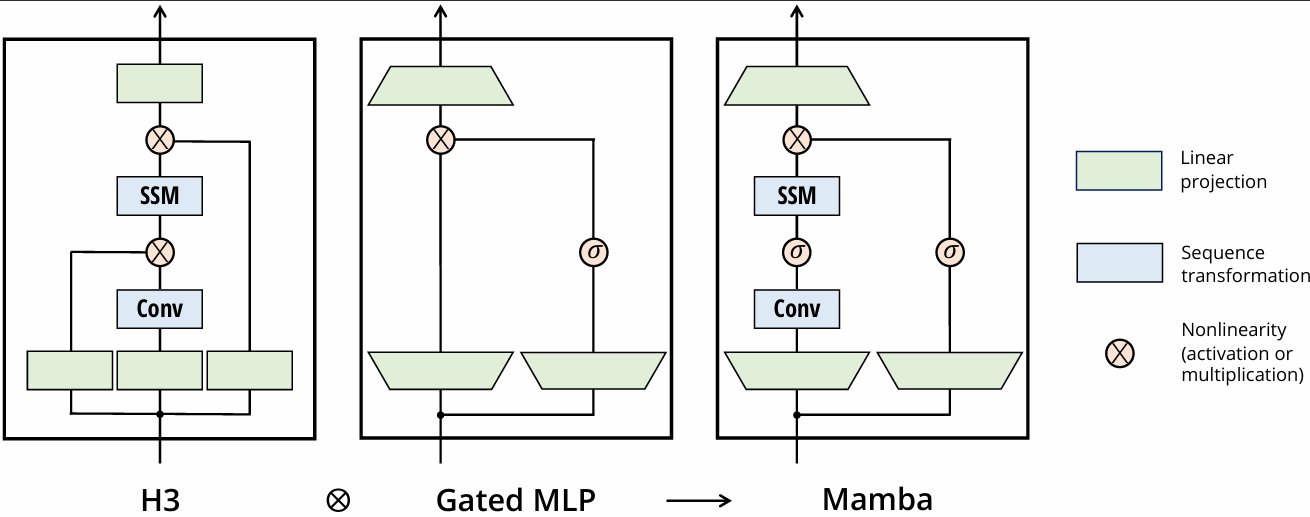
\includegraphics[width=\linewidth]{figures/h3_mlp_mamba.png}
    \caption{Architecture and the components of a Mamba block. Compared to the H3 block, Mamba replaces the first multiplicative gate with an activation function. Compared to the MLP block, Mamba adds an SSM to the main branch \cite{gu_mamba_2024}[Figure 3].} 
    \label{fig:h3_mlp_mamba}
\end{figure}



\subsubsection{\acrfull{vms}}
The \acrfull{vms} is a \acrfull{sota} implementation in the Papers with Code benchmark. It integrates a \acrlong{s6} optimized for long-range temporal dependencies and offers robust performance across various video event detection tasks. \cref{fig:mamba_ssm} shows the Mamba adoption they use to extend its performance into the video domain. The \acrfull{dbm} begins with distinct linear layers to separate forward- and backward-features. Then, both features pass through \acrshort{ssm} with bidirectional scanning. The features undergo two gating layers before they concatenate into an output token sequence \cite{li_videomamba_2024}. 

The \acrlong{vms} builds upon the ActionFormer transformer framework. It changes the transformers into Mamba blocks. \cref{fig:actionformer_architecture} shows how ActionFormer is designed. 

\begin{figure}
    \centering
    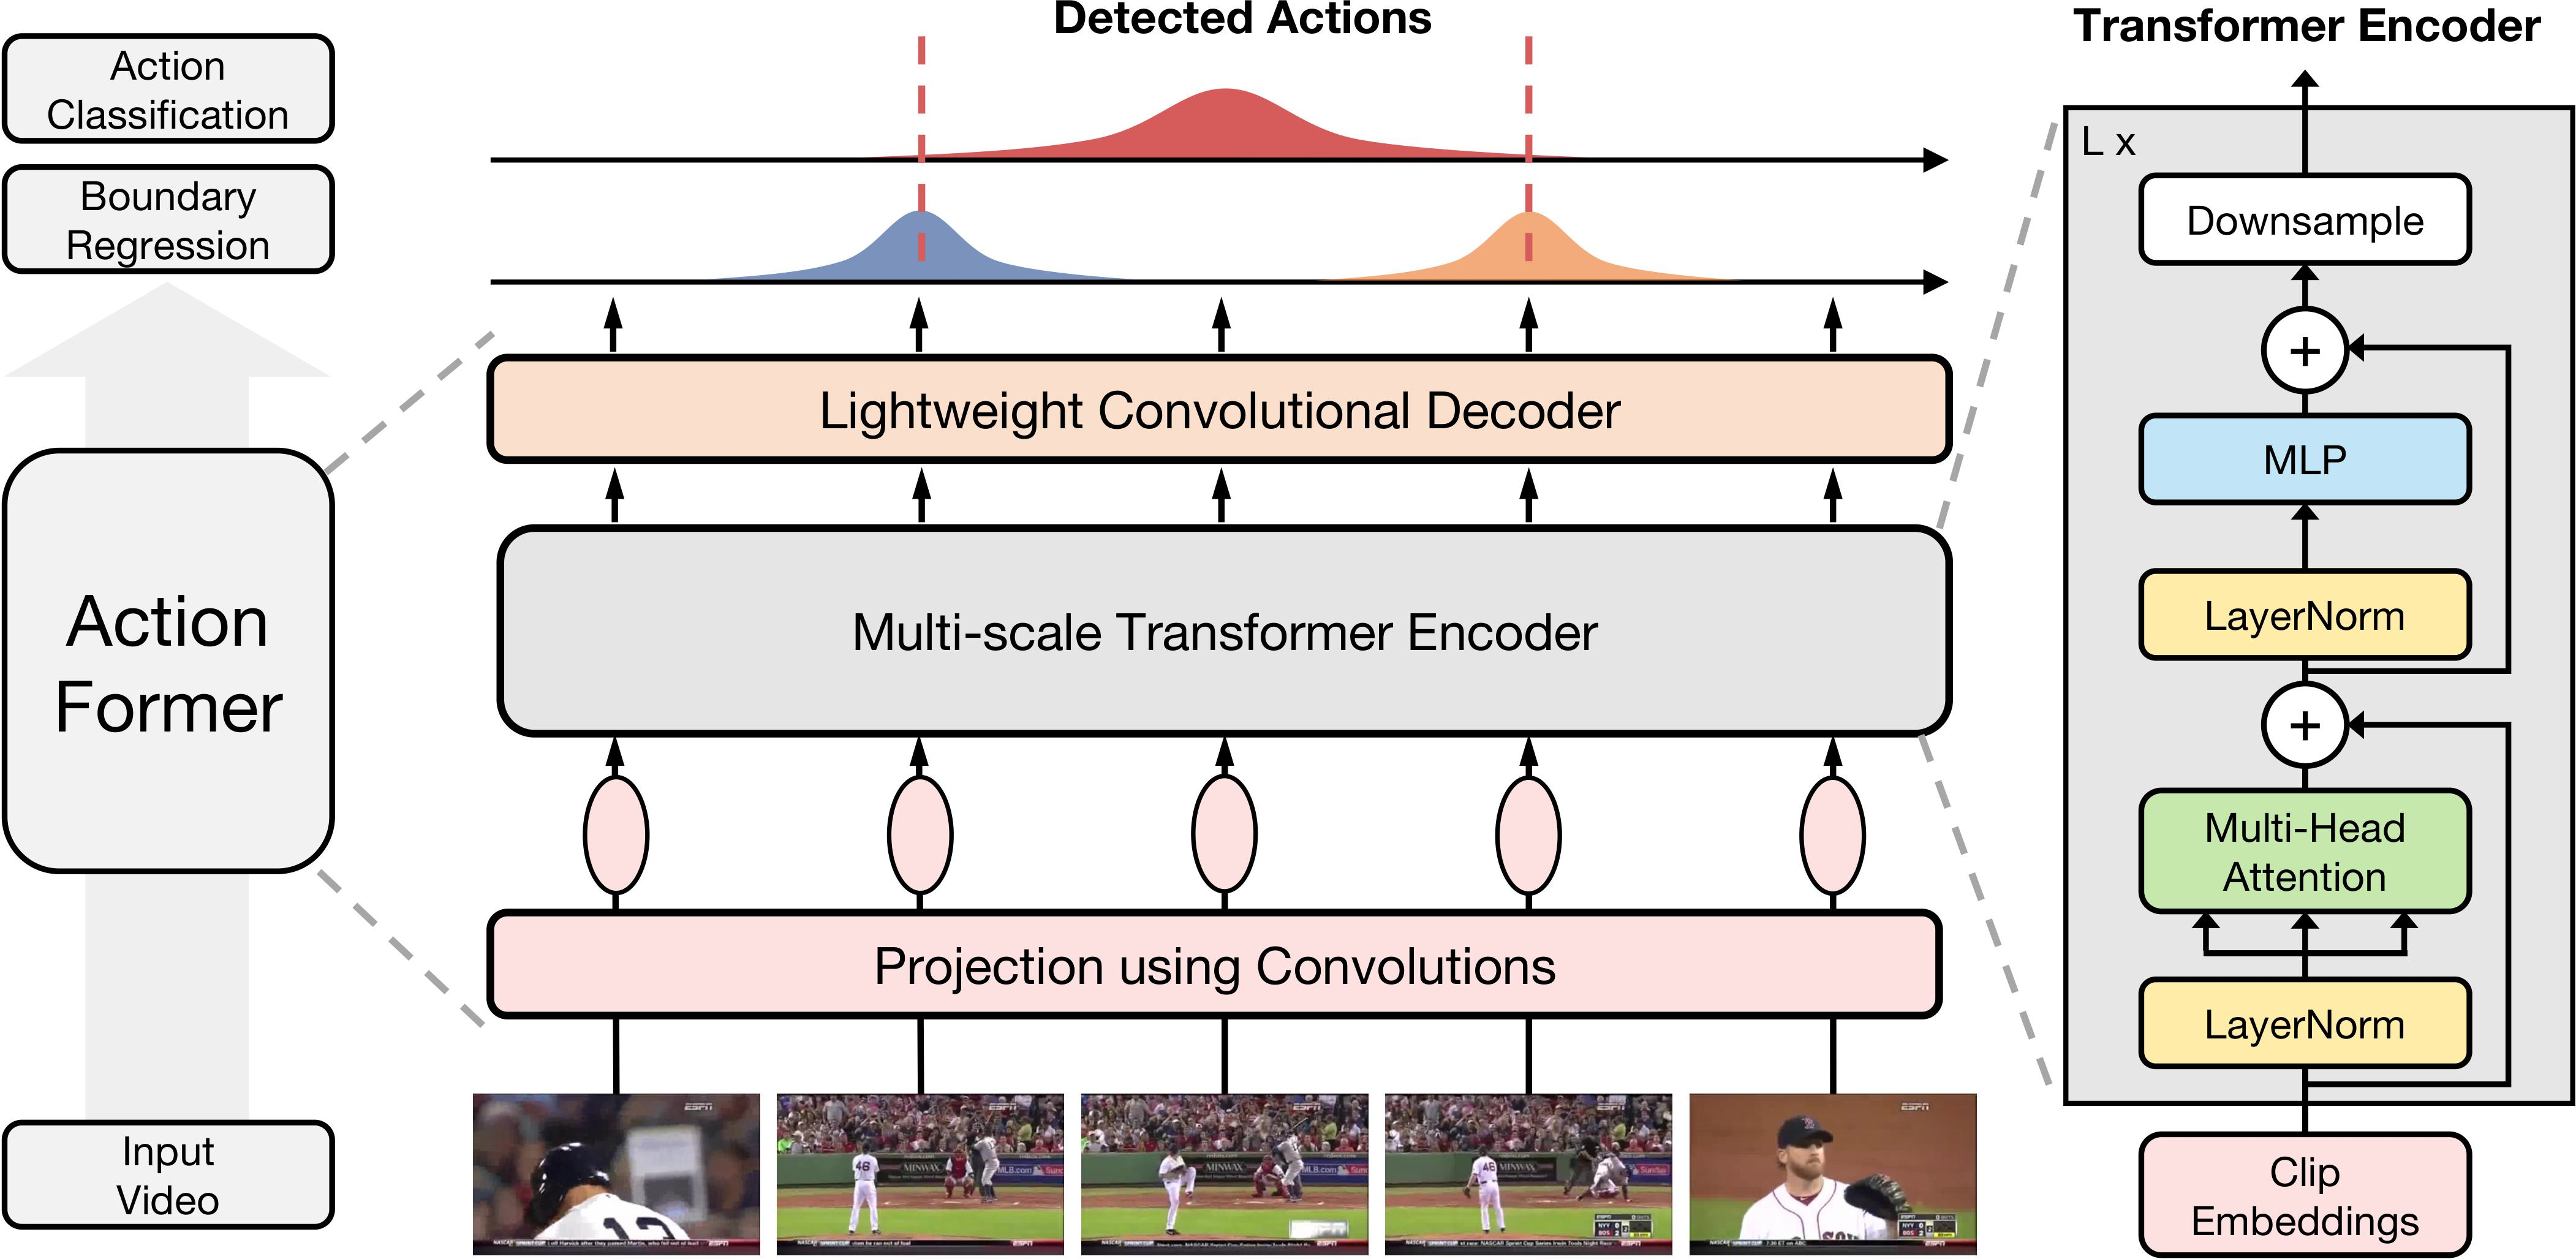
\includegraphics[width=1\linewidth]{figures/actionformer_architecture.jpg}
    \caption{Overview of the ActionFormer architecture \cite{zhang_actionformer_2022} . \acrshort{vms} switches the transformer encoders to Mamba blocks. }
    \label{fig:actionformer_architecture}
\end{figure}

\begin{figure}
    \centering
    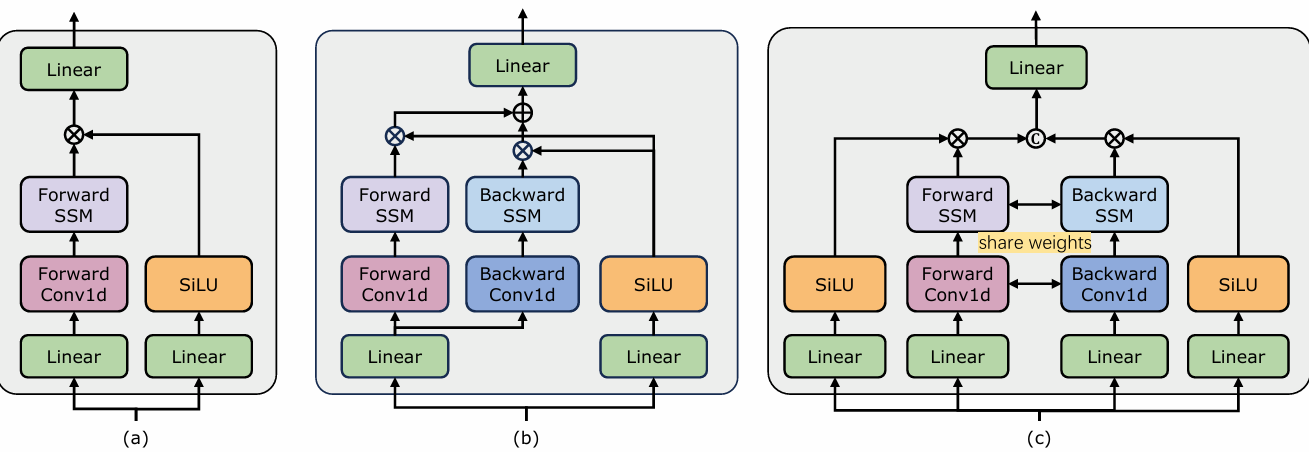
\includegraphics[width=1\linewidth]{figures/mamba_ssm.png}
    \caption{Three \acrshort{ssm} blocks. (a) is the vanilla Mamba block\cite{gu_mamba_2024}. (c) is the proposed \acrshort{dbm} block by \textcite{li_videomamba_2024}.}
    \label{fig:mamba_ssm}
\end{figure}

\subsubsection{RDFA-S6}
The RDFA-S6 architecture extends the \acrshort{vms} core with recurrent mechanisms. Empirical evaluations reveal that RDFA-S6 achieves slightly higher \acrlong{map} compared to \acrshort{vms}. The recurrent mechanisms indicate a slight improvement in performance in event localization benchmarks on THUMOS-14, ActivityNet, FineAction, and HACS. 

Although RDFA-S6 showed marginally improved accuracy, limited documentation hindered its adoption. Compared to the well-documented \acrlong{vms}, RDFA-S6 documentation lacked central elements, such as datasets. Consequently, \acrshort{vms} remained this study's primary model for empirical evaluation. 


\subsection{\acrfull{tdeed}}
\label{ssec:tdeed}

\acrfull{tdeed} is a deep learning architecture designed to address the challenge of \acrfull{pes} in sports videos. This model enhances token discriminability while utilizing multiple temporal scales, thereby ensuring high-resolution event localization. The architecture consists of three main components: a feature extractor, a temporally discriminant encoder-decoder, and prediction heads \cite{xarles_t-deed_2024}.

The feature extractor generates per-frame feature representations. It employs a RegNetY-based backbone with \acrfull{gsf} modules, integrating local temporal context while maintaining spatial information. Given an input frame sequence of shape \(\mathbb{R}^{L \times H \times W \times 3}\), the extracted feature representation is formulated as:

\[
z \in \mathbb{R}^{L/{k^j \times d} }
\]

The encoder-decoder architecture enables processing across multiple temporal scales, capturing events that require varying amounts of temporal context. The encoder enhances token discriminability using \acrfull{sgp} layers, which mitigate similarity issues commonly present in adjacent frames. The temporal dimension is downscaled through max-pooling, followed by an upsampling process in the decoder. Skip connections are integrated into the decoder using the \acrshort{sgp}-Mixer layer, aggregating features from different temporal scales while preserving fine-grained details.

The prediction head consists of a classification head and a displacement head. The classification head predicts event occurrences per frame using a softmax function, while the displacement head improves predictions by estimating the precise event frame within a given radius. The heads ensure potent event localization even when slight spatial or temporal differences exist.


\acrshort{tdeed} trains end-to-end using a multi-task loss. The loss comprises a weighted cross-entropy loss \(\mathcal{L}_c\) and a displacement loss \(\mathcal{L}_d\), defined as

\[
\mathcal{L} = \frac{1}{L}\sum_{l=1}^{L}\Big(\mathcal{CE}_{w}(y_l^{c},\hat{y}_l^c) + \operatorname{MSE}(y_l^{d},\hat{y}_l^d)\Big).
\]

Here, \(y_l^{c}\) is the one-hot encoding of the event in frame \(l\). The probability distribution at frame \(l\) is denoted by \(\hat{y}_l^c\). Similarly, \(y_l^{d}\) and \(\hat{y}_l^d\) represent the ground truth and predicted displacements, respectively.

The experiments use a T-DEED implementation adapted for the SoccerNet challenge. Videos are turned into pictures of each frame and stored offline, following the original method. Event spotting performance is evaluated using \acrlong{map}.


\section{Event Spotting Pipeline} 

\begin{figure}
    \centering
    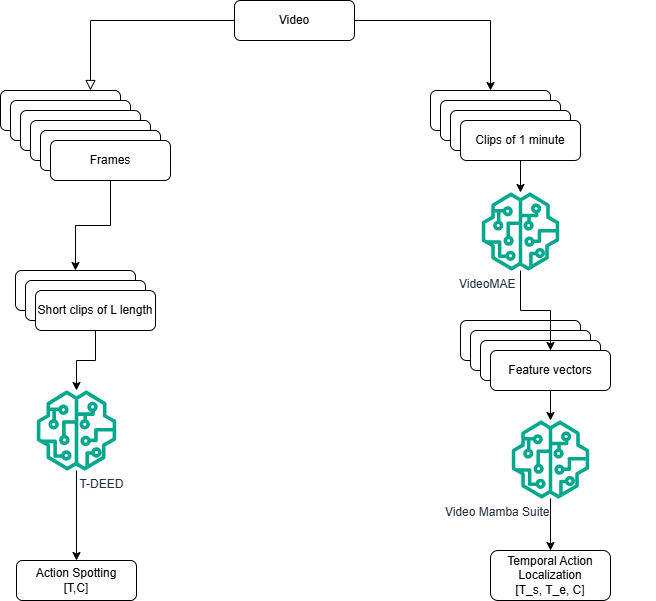
\includegraphics[width=0.75\linewidth]{figures/pipeline.png}
    \caption{The pipelines of the two models used in the thesis show how each model transforms the video. The \acrshort{tdeed} creates clips of 16 frames each, while \acrshort{vmae} creates a feature vector for each clip. The processed video is run through the model to infer a prediction.}
    \label{fig:pipeline}
\end{figure}

Both the \acrfull{tdeed} and \acrfull{vms} preprocess the full videos, as illustrated in \cref{fig:pipeline}. In the \acrshort{tdeed} preprocess pipeline, the system extracts all the frames from a video and saves them as image files locally. The model then reassembles these images into clips, with each frame receiving a token. During inference, the pipeline applies a 50\% overlap and \acrfull{snms} to maximize performance.

For the \acrshort{vms} pipeline, the process begins by splitting the video into 60-second-long clips. The last minute of each half may be shorter. The system infers these clips using \acrshort{vmae} and stores the feature vectors locally before \acrshort{vms} generates predictions. Additionally, \acrshort{vms} employs \acrshort{snms} and $topk$ as its postprocessing techniques.

The system logs all training and inference through \acrfull{wandb}, ensuring that configurations and hyperparameters are saved there. In the \acrshort{vms} pipeline, cropping serves as an augmentation technique. In contrast, \acrshort{tdeed} employs a variety of augmentation methods, including random cropping, random horizontal flip, Gaussian blur, color jitter, and mixup \cite{xarles_t-deed_2024}.

\section{Bayesian Hyperparameter Optimization}
\label{sec:bayesian_optimization}

\acrshort{wandb} sweeps perform Bayesian Optimization for efficient hyperparameter tuning. A Gaussian Process surrogate model was used to represent the validation \acrshort{map} as a function of the hyperparameters. Uniform and log-uniform priors were defined over each hyperparameter in the sweep configuration *.YAML file. The expected improvement function guided the selection of hyperparameter combinations. 70 trials were run in three iterations. The 70 runs were in parallel\footnote{All runs were run as individual training and had nothing to do with each other except the \acrshort{wandb} agent designing parameters.} across multiple \acrshort{gpu}s to explore the search space. All metrics and configuration parameters were logged to \acrshort{wandb}, enabling real-time monitoring and reproducibility. 


\section{\acrshort{vms} Evaluation Protocol}
\label{sec:eval_protocol}

When evaluating \acrshort{vms} performance, the 50\% \acrshort{map} criterion from the SoccerNet benchmark is adopted, which employs a $\pm1s$ tolerance window for event matching. Since the \acrshort{vms} model is validated against fixed‐length intervals of $L = 2\,$s, achieving $\mathrm{IoU}\ge0.5$ requires an overlap of at least $L/2 = 1s\,$.

Let $t^*$ denote the ground‐truth event time and $t_p$ the predicted center. The predicted interval is
\[
    [\,t_p - L/2,\;t_p + L/2\,]
    = [\,t_p - 1,\;t_p + 1\,].
\] 
The IoU condition
\[
    \mathrm{IoU}
    = \frac{\text{overlap}}{\text{union}}
    \;\ge0.5
    \quad\Longrightarrow\quad
    \text{overlap}\ge1
    \quad\Longrightarrow\quad
    |t_p - t^*|\le1
\]
ensures that the predicted center $t_p$ lies within one second of the actual event time.

Runtime was measured from \acrshort{wandb} logs, as the platform automatically records wall-clock time for each training run and from scripts. However, these values vary according to the assigned \acrshort{gpu} model. All measurements were standardized on a single A100 \acrshort{gpu} type to ensure fair comparisons. 
\section{Tools and Resources}
\label{sec:tools_and_resources}

\subsection{IDUN}
\label{ssec:idun}
Video processing pipelines demand substantial computational resources. IDUN is a faculty-operated system at \acrfull{ntnu} equipped with 234 NVIDIA \acrfull{gpu} accelerators (as of the 24th of April, 2025)\footnote{\url{https://www.hpc.ntnu.no/idun/}}. Although IDUN is not \acrshort{ntnu}'s central supercomputer, its nodes, featuring Tesla H100, A100, V100, and P100 \acrshort{gpu}s, with up to 80 GB of RAM, provided the necessary throughput for feature extraction and model training. The feature extraction partitions a full match into fixed-duration clips and distributes workloads across multiple \acrshort{gpu}s via data-parallel training to mitigate queuing delays.


Due to the high memory requirements of the \acrfull{tdeed} and software requirements of the \acrfull{s6} framework, all experiments run on IDUN nodes. Attempts to train on \acrshort{gpu}s with 16 GB of memory trigger out-of-memory errors with \acrshort{tdeed}. Moreover, MAMBA \acrshort{s6} requires specific CUDA versions and matching libraries, which older driver stacks do not support. Model development and evaluation are restricted to nodes that meet these hardware and software requirements to ensure stable training and reproducible results. 

\subsection{\acrfull{wandb}}
\label{ssec:wandb}

The acrlong{wandb} platform streamlined the management and reproducibility of the training experiments. Hyperparameters are logged automatically using \acrshort{wandb}'s Python client, as are training and validation metrics, model checkpoints, and \acrshort{gpu} utilization statistics. A dashboard enables real-time monitoring of experiments, as well as direct and live comparison of runs. \acrshort{wandb}'s automated hyperparameter conducted hyperparameter searches. Coordinated sweeps logged performance metrics and visualized the results. 

\subsection{Bayesian Hyperparameter Search}

Bayesian optimization uses probability to tune hyperparameters. It balances exploring new hyperparameter values with exploiting known good ones. The method uses a Gaussian Process as a surrogate model to predict the \acrlong{map} performance metric.

The optimization process follows these steps:
\begin{itemize}
    \item \textbf{Surrogate Model}: A probabilistic model estimates the objective function based on previous evaluations.
    \item \textbf{Acquisition Function}: Determines the next hyperparameter set to evaluate by optimizing a function such as Expected Improvement or Upper Confidence Bound.
    \item \textbf{Evaluation and Update}: The chosen hyperparameters are tested, and the surrogate model is updated with new information.
    \item \textbf{Iteration}: The process repeats for a set number of runs.
\end{itemize}

Bayesian optimization is beneficial for deep learning models because testing each hyperparameter set requires significant computing power. It utilizes probability to determine the optimal hyperparameters, thereby reducing the number of tests needed.


\subsection{Comparing Correlation and Importance}


Correlation identifies linear dependencies between the parameter and output, while importance aims to determine the likelihood of a parameter affecting production. Importance seeks to find the parameters that are most likely to have an impact when tuned. Correlations are sensitive to outliers and may not accurately detect polynomial relationships. Importance can capture more complex relations, as it accounts for interactions between hyperparameters. 

\subsection{Anaconda and pip}
\label{ssec:conda_pip}
Conda manages the Python environments. However, all packages, including CUDA-enabled PyTorch builds, were installed via Pip to follow recent PyTorch recommendations. Those recommendations favor Pip over conda for \acrshort{gpu} support.

\section{Environment} 

Each model had a unique environment. Python was installed on Conda virtual environments, while Pip managed packages within the environments. \acrshort{vms} relied on the GNU Compiler Collection (GCC) to install hardware-specific algorithms to speed up training. Causal Conv1D \footnote{\url{https://github.com/Dao-AILab/causal-conv1d}} and Mamba \footnote{\url{https://github.com/state-spaces/mamba}}  were installed in the \acrshort{vms} environment.